\documentclass[11pt]{article}
\usepackage{euscript}

\usepackage{amsmath}
\usepackage{amsthm}
\usepackage{amssymb}
\usepackage{epsfig}
\usepackage{xspace}
\usepackage{color}
\usepackage{url}
\usepackage[shortlabels]{enumitem}


%%%%%%%  For drawing trees  %%%%%%%%%
\usepackage{tikz}
\usetikzlibrary{calc, shapes, backgrounds}

%%%%%%%%%%%%%%%%%%%%%%%%%%%%%%%%%
\setlength{\textheight}{9in}
\setlength{\topmargin}{-0.600in}
\setlength{\headheight}{0.2in}
\setlength{\headsep}{0.250in}
\setlength{\footskip}{0.5in}
\flushbottom
\setlength{\textwidth}{6.5in}
\setlength{\oddsidemargin}{0in}
\setlength{\evensidemargin}{0in}
\setlength{\columnsep}{2pc}
\setlength{\parindent}{1em}
%%%%%%%%%%%%%%%%%%%%%%%%%%%%%%%%%


\newcommand{\eps}{\varepsilon}

\renewcommand{\c}[1]{\ensuremath{\EuScript{#1}}}
\renewcommand{\b}[1]{\ensuremath{\mathbb{#1}}}
\newcommand{\s}[1]{\textsf{#1}}

\newcommand{\E}{\textbf{\textsf{E}}}
\renewcommand{\Pr}{\textbf{\textsf{Pr}}}

\title{Homework 1 - Decision Trees
	\footnote{\s{CS 6350 Machine Learning; \;\; Spring 2024 \hfill
			Instructor: Vivek Kumar, University of Utah}
	}
}
\author{Cristian Tapiero}

\begin{document}
	\maketitle
	
	
	
	
	
	%%%%%%%%%%%%%%%%%%%%%%%%%%%%%%%%%%%%%%%%%%%%%%%%%%%%
	%%%%%%%%%%%%%%%%%%%%%%%%%%%%%%%%%%%%%%%%%%%%%%%%%%%%
	%%%%%%%%%%%%%%%%%%%%%%%%%%%%%%%%%%%%%%%%%%%%%%%%%%%%
	\section{Problem 1}
	1.
	\begin{enumerate}[(a)] % (a), (b), (c), ...
		\item the total number of rows for the given attributes is $3\times3\times2\times2 = 36.$  
		So if we consider the values to be binary  there are $2^{36}$ possible functions.
		
		The number of functions that are consistent with the table given is $2^{8} = 256$
		
		\item Entropy is defined as $$H(S) =-p_+ log (p_+)-p_- log(p_-)$$
		
		Because $p_+ = p_- = 1/2$ Therefore, $H(S) = 1$
		
		\item Gain is defined as: $$\textit G(S,A) = Entropy(S) - \sum_{v\in Values(A)} \frac{|S_v|}{|S|} Entropy(S_v)$$ 
		
		As an example of the calculation, select A as the attribute Variety.
		$$\textit A = \{Alphonso,Keith,Haden\}$$
		
		First we calculate the Entropy for each of the subsets of the attribute Variety:
		
		$$\textit Entropy(Alphonso) = - \frac{1}{2}log(\frac{1}{2}) - \frac{1}{2}  log(\frac{1}{2}) = 1$$
		
		$$\textit Entropy(Keith) = -\frac{1}{3}log -\frac{2}{3} log(\frac{2}{3}) = 0.9118$$
		
		$$\textit Entropy(Haden) = -1log(1) - 0 log(0) = 0$$
		
		Then we compute the average part of the equation or the expected Entropy:
		$$\textit E(Entropy_{variety}) = 1 \times \frac{4}{8} + 0.918\times \frac{4}{8} + 0 \times \frac{1}{8} = 0.844$$
		
		Finally we calculate the Gain by subtracting the above value from the total entropy of the data set:
		$$\textit G(S,Variety) =  1 - 0.844 = 0.156 $$
		
		a similar procedure is applied to calculate the remaining gains for the other attributes given. The remaining results are presented in table 1.
		
		\begin{align}
			\begin{array}{cc}
				\hline \hline \text { Feature } & \text { Information Gain } \\
				\hline 
				Variety & 0.156  \\
				Color & 0.062  \\
				Smell & 0.189  \\
				Time & 0.049  \\
				\hline
			\end{array}
		\end{align}
		
		\begin{center} Table 1. Information Gain \end{center}
	
	\item I would use the Smell attribute to construct the root of the tree because is the highest value in table 1.
	\item The following tree represents the data given, choosing Smell as the root.
	\begin{center}
	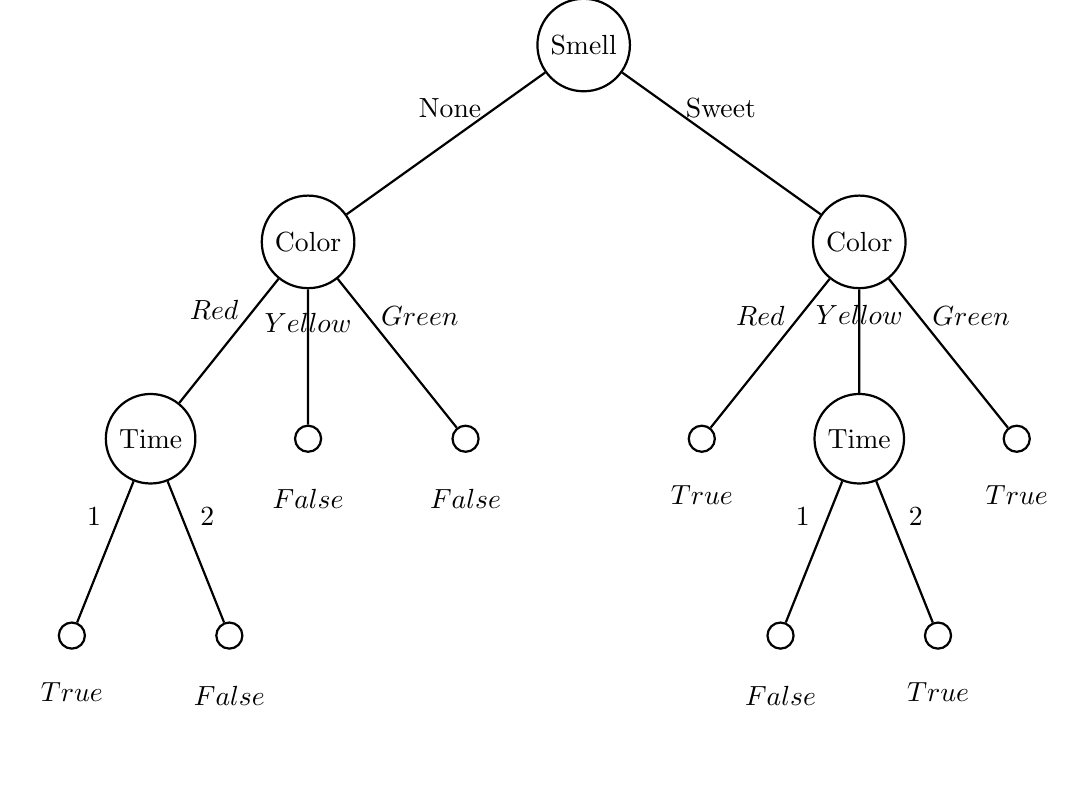
\begin{tikzpicture}[
		scale = 1, transform shape, thick,
		every node/.style = {draw, circle},
		grow = down,  % alignment of characters
		level 1/.style = {sibling distance=7cm},
		level 2/.style = {sibling distance=2cm}, 
		level distance = 2.5cm
		]
		\node (Start) { Smell} 
		child {   node (A) {Color}
			child { node (B) {Time} child{node (K) {}} child{node (J) {}}}
			child { node (C) {} }
			child { node (D) {}}
		}
		child {   node (E) {Color}
			child { node (F) {}}
			child { node (G) {Time} child{node (L) {}} child{node (M) {}}}
			child { node (H) {}}
		};
		
		
		% Put probability on edges
		\begin{scope}[nodes = {draw = none}]
			\path (Start) -- (A) node [near start, left]  {None};
			\path (A)     -- (B) node [near start, left]  {$Red$};
			\path (B)     -- (K) node [near start, left]  {$1$};
			\path (B)     -- (J) node [near start, right]  {$2$};
			\path (A)     -- (C) node [near start] {$Yellow$};
		    \path (A)     -- (D) node [near start,right] {$Green$};
			\path (Start) -- (E) node [near start, right] {Sweet};
			\path (E)     -- (F) node [near start, left]  {$Red$};
			\path (E)     -- (G) node [near start] {$Yellow$};
			\path (G)     -- (L) node [near start,left] {$1$};
			\path (G)     -- (M) node [near start,right] {$2$};
			\path (E)     -- (H) node [near start, right] {$Green$};
			\begin{scope}[nodes = {below = 4pt}]

				\node at (C) {$False$};
				\node at (D) {$False$};
				\node at (F) {$True$};
				\node at (H) {$True$};
				\node at (K) {$True$};
				\node at (J) {$False$};
				\node at (L) {$False$};
				\node at (M) {$True$};
			\end{scope}
		\end{scope}
	\end{tikzpicture}
	\end{center}
	
	\begin{center} Figure 1. Decision Tree \end{center}
	
	$\newline$
		\item using the decision tree on figure 1 we get the following predictions listed as a the last column in table 2
	
	\begin{align}
		\begin{array}{cccccc}
			\hline \hline \text { Variety } & \text { Color } & \text { Smell } & \text { Time } & \text { Ripe? } & \text { Predicted Label } \\
			\hline 
			Alphonso & Green & Sweet & Two & True & True \\
			Keitt & Red & Sweet & One & False  & True\\
			Haden & Yellow & None & Two & True &False\\
			\hline
		\end{array}
	\end{align}
	
	\begin{center} Table 2. Predicted Values \end{center}
	
	We can calculate the Accuracy of the classifier as follows:
	
	$$Accuracy =( 
	\displaystyle\frac{\text{ Number of Correct Predictions}}{\text
		{Number of Predictions}}) \times 100$$
	
	Therefore, only having 1 correct prediction give an accuracy of about 33.33x\%
	
	

	\end{enumerate}
2.
	\begin{enumerate}[(a)]
		\item  the New Information Gain is defined as: $$\textit G(S,A) = MajorityError(S) - \sum_{v\in Values(A)} \frac{|S_v|}{|S|} MajorityError(S_v)$$ 
		where MajorityError is defined as:
		$$\textit MajorityError(S) = 1 - max_ip_i$$ 
		$$\textit MajorityError(S_v) = 1 - max_ip_{i,v}$$ 
		
		
		\end{enumerate}
\end{document}
